\documentclass[12pt,american]{article}
\usepackage[T1]{fontenc}
\usepackage{fourier}
\usepackage[hidelinks]{hyperref}
\usepackage{babel}
\usepackage[babel]{microtype}
\usepackage[babel]{csquotes}
\usepackage[journal={IEEE Transactions on Mobile Computing},
			manuscript={TMC-2025-02-0445},
			editor={editors}]{reviewresponse}
\usepackage{fancyhdr}
\usepackage{lastpage}
\usepackage[a4paper,total={160mm,245mm},left=25mm,top=25mm]{geometry}
\renewcommand{\headrulewidth}{0pt}
\renewcommand{\footrulewidth}{.5pt}
\usepackage[shortlabels]{enumitem}
\newlist{detail}{itemize}{3}
\setlist[detail, 1]{label=\textbullet,leftmargin=21pt,nosep}
% \usepackage[backend=biber,style=ieee,dashed=false,url=true,isbn=false,defernumbers=true,refsection=section]{biblatex}
\usepackage[backend=biber,refsection=section,style=ieee,url=true,isbn=false,dashed=false]{biblatex}
\usepackage{romannum}
\usepackage{amsmath, amsfonts}
\usepackage{textcomp}
\usepackage{caption}
\usepackage[caption=false,font=normalsize,labelfont=sf,textfont=sf]{subfig}
\usepackage{booktabs}
\usepackage{array}

\newcommand{\ie}{\emph{i.e., }}
\newcommand{\eg}{\emph{e.g., }}
\newcommand{\etal}{\emph{et al.}}

% \bibliography{literature.bib}
\addbibresource{literature.bib}


\title{Optimizing Joint Speed and Altitude Schedule for UAV Data Collection in Low-Altitude Airspace}
\author{Yiqian Wang, Jianping Huang, Feng Shan, Yuming Gao, Runqun Xiong and Junzhou Luo}


\begin{document}
\maketitle

% Cover Letter
\thispagestyle{empty}
\noindent Dear \editorname,

Please find enclosed the revised version of our previous submission entitled \enquote{\thetitle} with manuscript number \manuscript. We would like to thank you and the reviewers for the valuable comments which help improving the quality of our manuscript.
In this revision, we have carefully addressed the reviewers' comments. A summary of main modifications and a detailed point-by-point response to the comments from Reviewers 1 and 3 (following the reviewers' order in the decision letter) are given below.

\vspace{8em}

\noindent Sincerely,

\noindent\theauthor

\vfill
\textbf{Note:} To enhance the legibility of this response letter, all the editor's and reviewers' comments are typeset in boxes. Rephrased or added sentences are typeset in color. The respective parts in the manuscript are highlighted to indicate changes.
\pagenumbering{arabic} % 改为阿拉伯数字页码
\setcounter{page}{0}
\pagestyle{fancy}
\fancyfoot[R]{\thepage\ / \pageref{LastPage}}
\fancyfoot[L]{Response Letter for \manuscript}
\fancyfoot[C]{\ }
% Response to Editor
\editor

% todo complete

\begin{metacomment}
	Clearly differentiate the contributions from prior works.
\end{metacomment}
\begin{metaresponse}%[We appreciate your handling of the review process.]
\end{metaresponse}

\begin{metacomment}
	Address limitations for practical application of the algorithm.
\end{metacomment}
\begin{metaresponse}
	
\end{metaresponse}

\begin{metacomment}
	Validate the claim of ``near-optimal performance.''
\end{metacomment}
\begin{metaresponse}
	
\end{metaresponse}

\begin{metacomment}
	Test SSF-ACO and SSF-ACO-Online under network dynamics (e.g., node mobility).
\end{metacomment}
\begin{metaresponse}
	
\end{metaresponse}

\begin{metacomment}
	Explain the rationale behind heuristic factor selection.
\end{metacomment}
\begin{metaresponse}
	
\end{metaresponse}

\begin{metacomment}
	Include more comprehensive experimental validation.
\end{metacomment}
\begin{metaresponse}
	
\end{metaresponse}

\begin{metacomment}
	Extend the discussion of related literature for completeness.
\end{metacomment}
\begin{metaresponse}

\end{metaresponse}
% Reviewer 1
\reviewer

\begin{revcomment}
	This paper fails to justify the selection of heuristic factors $(\alpha, \beta)$ in SSF-ACO. You should conduct grid search experiments to demonstrate parameter sensitivity or cite theoretical foundations for ACO parameter tuning.
\end{revcomment}
\begin{revresponse}
	Thank you for the comment.
	We performed a grid-search over representative combinations of the pheromone exponential factor $\alpha\in\{1,2,3,4\}$ and heuristic exponential factor $\beta\in\{0,1,2,3,4\}$ to access parameter sensitivity as shown in Figure~\ref{fig:cali}.
	The algorithm's performance under $\beta=0$ is significantly worse than performance for other parameter combinations. $\beta=0$ eliminates the use of heuristic information, resulting in purely random exploration during the initial iterations and thus poor performance.
	The results also indicate that the configuration $\alpha=1,\beta=2$ consistently achieves the minimum energy consumption. Accordingly, we adopted $\alpha=1,\beta=2$ in all simulation experiments.
	\begin{figure}[h]
		\centerline{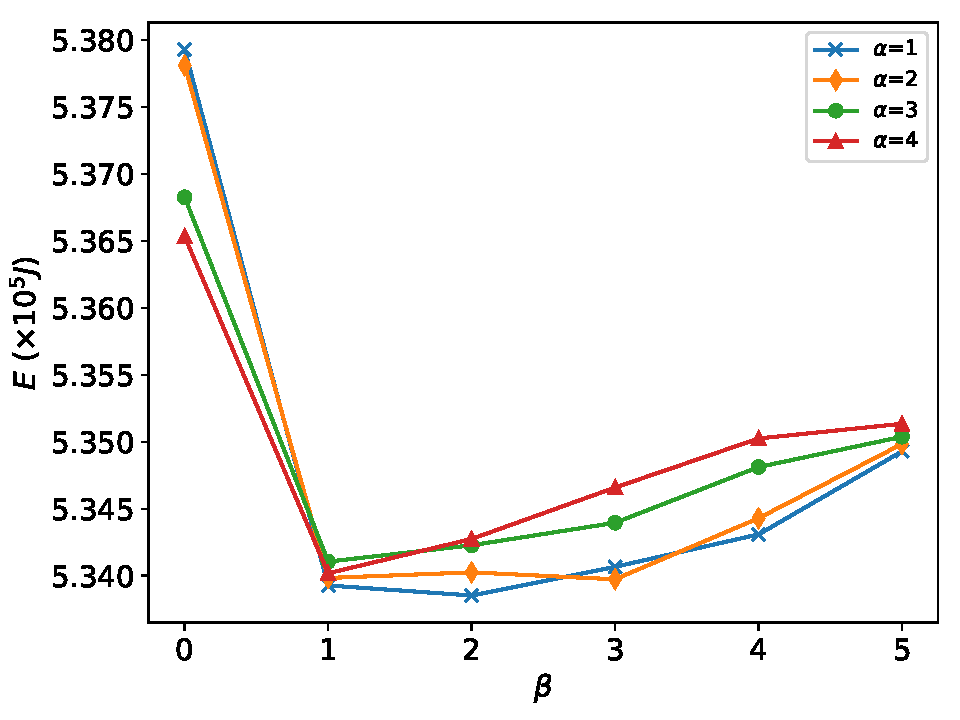
\includegraphics[width=.5\textwidth]{fig/cali.pdf}}
		\caption{Performance of SSF-ACO across different $(\alpha,\beta)$ combinations.}
		\label{fig:cali}
	\end{figure}
\end{revresponse}

\begin{revcomment}
	Current experiments only cover small-scale scenarios ($\leq 30$ nodes), it should extend to more nodes to should the scalibility of algorithm.
\end{revcomment}
\begin{revresponse}
	Thank you for the suggestion.
	Our algorithms are designed with scalability and is capable of handling larger-scale problems.
	To further verify its scalability, we extended the evaluation to include scenarios involving 35 and 40 ground sensor nodes. The updated results are illustrated in Figure~\ref{fig:40nodes}, which is identical to Figure~8a in the manuscript. The results demonstrate that the proposed algorithms continue to exhibit superior performance even in larger-scale scenarios.
	\begin{figure}[h]
		\centerline{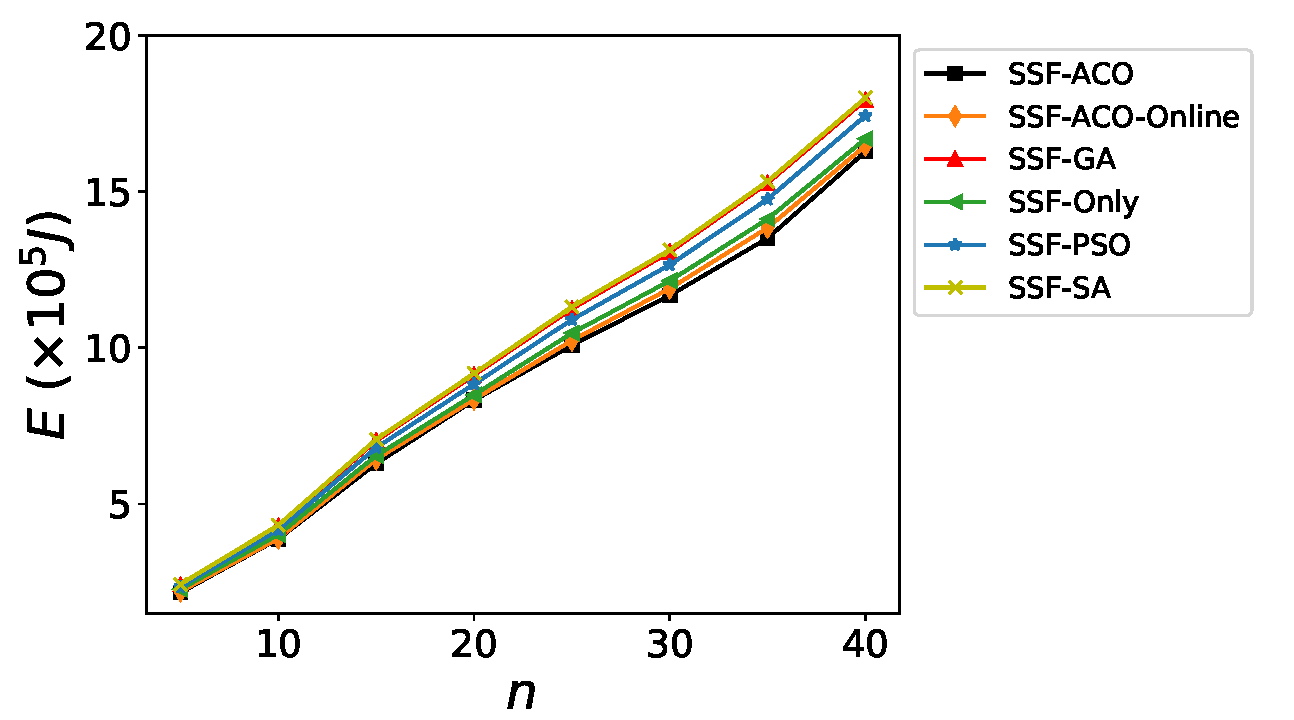
\includegraphics[width=.6\textwidth]{fig/exp_number_40_legend.pdf}}
		\caption{Algorithm performance comparisons in UAV energy consumption under varying numbers of sensors.}
		\label{fig:40nodes}
	\end{figure}
\end{revresponse}

\begin{revcomment}
	The assumptions of linear GN deployment and complete GN knowledge are restrictive and not sufficiently justified. Please provide a detailed discussion of the assumptions, including their implications for real-world applicability and potential extensions.
\end{revcomment}
\begin{revresponse}
	We appreciate the reviewer's comment regarding the assumptions of linear GN deployment and complete GN knowledge.
	We would like to provide additional details about GN deployment and GN knowledge, as well as a discussion of these assumptions in Section 6 of our revised manuscript.

	\textbf{Linear GN deployment.}
	The linear configuration of GNs represents a reasonable and commonly utilized setup in real-world systems.
	This deployment pattern often arises in infrastructure monitoring scenarios.
	For instance, in the power line~\cite{powerline,transmission-line}, UAVs are dispatched to autonomously collect data from sensors on the transmission tower.
	Similarly, in the oil and gas industry~\cite{pipeline}, UAVs are used to fly along pipelines for inspection activities.
	In addition, sensors can be deployed along rivers~\cite{river} and coasts~\cite{coast} to capture diel and seasonal fluctuations, with the purposes of ecological monitoring, flood warning, and scientific research.

	In fact, the effectiveness of such linear GN deployment has already been demonstrated in industrial applications to reduce costs, improve work efficiency, and avoid hazardous manual tasks.
	For instance, DJI has successfully implemented UAV-enabled solutions in scenarios such as long-distance pipelines~\cite{DJI-pipeline}, power transmission line in plateau regions~\cite{DJI-powerline}, and river ecosystems~\cite{DJI-river}, where the UAV trajectories can be regarded as linear or the combination of multiple straight-line segments.

	\textbf{Complete GN knowledge.}
	Sensor knowledge mainly includes information such as position, amount of data to be collected, transmission rate, and data transmission range.
	(1) In the online problem, each sensor has an additional control communication range, which covers a larger area than the data transmission range.
	When the UAV enters the sensor's control communication range, it can detect the sensor and receives a response containing information such as the amount of data and the sensor's position.
	We have explained this process in the revised manuscript as shown below.
	(2) There is a proportional relationship between the radius of the data transmission range and the control communication range.
	Based on the distance between the sensor and the UAV at the moment the response is received, the radius of the data transmission range can be estimated.
	(3) The sensor position is fixed, and thus, it can be obtained during the initial deployment and periodic maintenance. This allows for the calibration of sensor positions.
	\begin{changes}
		The UAV keeps broadcasting `Probe' message during the flight to detect sensors. Once receiving the `Probe' message, the sensor sends back an `ACK' message, which includes its position, the amount of data, and transmission characteristics. Note that each sensor sends `ACK' message only once. This partial information availability fundamentally changes the nature of our optimization problem, requiring real-time 
		decision-making based on local information.
	\end{changes}
\end{revresponse}

\begin{revcomment}
	Could the proposed models and algorithms be adapted for 3D GN layouts?
\end{revcomment}
\begin{revresponse}
	Thanks for your comment.
	Our current focuses on the linear (2D) GN distribution, including power transmission lines, roads, pipelines, river and coast. By integrating advanced trajectory planning methods, our algorithms can be extended to 3D GN layout.

	Specifically, we first apply a trajectory planning algorithm to optimize the UAV's flight path and avoid collisions.
	The area of UAV trajectory planning and collision avoidance has been extensively studied in recent years.
	The distance travelled from the starting point to any location along the trajectory is treated as the horizontal coordinate of that location.
	Along this trajectory, we can then use SSF-ACO algorithm to jointly optimize speed and altitude scheduling.
	
	Although promising, this approach to extending the 3D GN layout remains subject to certain limitations.
	Jointly optimizing the 3D trajectory and speed scheduling is expected to have a better performance.
	Furthermore, the increased computational complexity associated with 3D scheduling problems presents additional challenges.
	However, these issue fall within a broader area that extends beyond the focus of the current work.
	Addressing them remains also one of our future research directions.
	In this work we concentrate on the optimization of speed and altitude scheduling, and demonstrate compatibility with existing trajectory planning algorithms.
\end{revresponse}

\begin{revcomment}
	Some statements have inconsistent tenses (e.g. ``Our previous work [20] investigated...''). vs. (``we propose...''), need to unify the full text tense; The reference format should be checked according to IEEE standards (e.g. URL references [6] are not standardized).
\end{revcomment}
\begin{revresponse}
	Thank you for the comment.
	We have carefully reviewed the tense usasge throughout the manuscript and corrected the inconsistent expressions to ensure consistency. Additionally, we have standardized the website reference format according to IEEE Reference Guide.
\end{revresponse}

\printpartbibliography{powerline,pipeline,transmission-line,river,coast,DJI-powerline,DJI-pipeline,DJI-river}

% Reviewer 2
\reviewer

\begin{revcomment} % \label{cmt:work-not-good}
	The computational latency of SSF-ACO-Online needs justify.
\end{revcomment}
\begin{revresponse}
	Thank you for the comment.
	% todo 运行时间的实验数据
\end{revresponse}

\begin{revcomment}
	Alg. 4 does not specify the specific implementation of ``Roulette-Wheel-Selection'', which needs to supplement pseudocode or reference standard methods.
\end{revcomment}
\begin{revresponse}
	Thanks for your suggestion.
	The classic Roulette wheel selection method is applied, and we have added a brief description of the Roulette-Wheel-Selection method in the revised manuscript.
	\begin{changes}
		Specifically, in \textbf{Roulette-Wheel-Selection}, the vertex $(\varphi+1, j')$ is selected if $\sum_{j''=0}^{j'-1}{p(\varphi,j,j'')}\leq \text{rand}() < \sum_{j''=0}^{j'}{p(\varphi,j,j'')}$, where $\text{rand}()$ generates a random number in $[0,1)$.
	\end{changes}
\end{revresponse}

\begin{revcomment}
	The vertical energy consumption is assumed to be linear related to the altitude difference, which seems oversimplified, more justification is needed.
\end{revcomment}
\begin{revresponse}
	Thanks for the comment.
	Research~\cite{vertical-assumption} serves as the theoretical basis for this ``linear assumption''.
	According to~\cite{vertical-assumption}, the following equation fits well with the theoretical derivation,
	\begin{equation}
		p_V = c_{0,V} + c_{1,V}v + c_{2,V}v^2,
	\end{equation}
	where $p_V$ is the vertical power consumption, $c_{0,V}$, $c_{1,V}$ and $c_{2,V}$ are coefficients, and $v$ is the climbing or descending speed of the UAV.
	In our manuscript, we assume that the UAV climbs or descends at a constant speed and flies in a stable environment.
	Therefore, the vertical power consumption is constant.
	For a certain altitude difference $\Delta h$, the vertical energy consumption is $E_V=\frac{p_V\Delta h}{v}$, which supports the ``linear assumption''.
	Furthermore, similar assumptions have also been adopted in previous research~\cite{mgh}.
\end{revresponse}

\begin{revcomment}
	The difference between the transmission range model of Equation (17) and literature [35] is not fully explained, and the improvement points or advantages need to be clearly defined.
\end{revcomment}
\begin{revresponse}
	
\end{revresponse}

\begin{revcomment}
	What is the purpose of presenting Equation (18)?
\end{revcomment}
\begin{revresponse}
	Thans you for the comment.
	Equation (18) in the original manuscript was included to provide a quantitative description of the data transmission range's width.
	To retain a more holistic presentation, we have modified the expression.
	\begin{changes}
		The width and height of the range are linearly related to the coefficients $C_W$ and $C_H$, respectively.
		And the quantitave relationship can be found in Appendix F of the supplementary material.
	\end{changes}
\end{revresponse}

\begin{revcomment}
	There are too many curves in Figure 8 and the colors are similar, so it is difficult to distinguish them. It is suggested to optimize the color matching or add mark symbols
\end{revcomment}
\begin{revresponse}
	Thanks for your suggestion.
	We have revised the color scheme and marker symbols to make the curves in Figure 8 in the revised manuscript, and also adjusted the layout of it to improve clarity.
	% todo 新图复制过来
\end{revresponse}

\begin{revcomment}
	The dynamic nature of the sensor is not considered, such as movement, inaccurate position, failure and other problems.
\end{revcomment}
\begin{revresponse}
	We appreciate the reviewer's comment on the dynamics of sensors, which highlights important aspects that could influence the effectiveness the UAV scheduling.
	In the following, we will discuss the ground nodes (GNs) mobility, inaccurate position, failures, and unstable communication environment.

	\textbf{GN mobility.}
	GN mobility is an important factor in various UAV-assisted systems.
	However, our current work focuses on data collection from stationary sensors.
	In the scenarios we consider, the sensors are fixed in the environment to monitor infrastructures or natural conditions.
	Admittedly, a number of existing studies~\cite{GNmob1, GNmob2, GNmob3, GNmob4} have investigated GN mobility. %, primarily in the context of UAV-assisted task offloading or crowd sensing.
	In these studies, GNs typically refer to mobile user devices with significant movement, such as user-carried devices~\cite{GNmob1,GNmob2} or vehicles~\cite{GNmob3,GNmob4}, which are fundamentally different from the stationary GNs considered in our work.

	\textbf{Inaccurate position.}
	The proposed algorithm relies on the precise sensor positions.
	However, the inaccurate sensor localization leads to discrepancies between the UAV scheduling and actual environment.
	In our future, we intend to employ more advanced relative positioning techniques to reduce localization inaccuracy and incorporate error-tolerant strategies to improve the system's robustness and reliability.

	\textbf{Failures.}
	Failures may occur either before or during data transmission.
	Failures before transmission will result in the sensor being undetectable by the UAV.
	On the other hand, failures during the transmission process will lead to a disruption in the connection between the UAV and the sensor.
	The UAV will attemp to reconnect and, after reaching the maximum number of reconnection attempts, will abandon the connection.
	Regardless of whether reconnection is successful, the scheduling will be re-planned to ensure energy efficiency.
	% todo 在论文online那节加一段描述

	\textbf{Unstable communication environment.}
	The changes in the communication environment may lead to fluctuations in the transmission rate.
	When the UAV first detects the sensor, it will receive the sensor's guaranteed minimum transmission rate included the sensor's `ACK' message.
	When the guaranteed transmission rate is not met, the UAV's speed and altitude scheduling will be re-planned by our algorithm to adapt to the environment changes. 

\end{revresponse}

\begin{revcomment}
	Some minor suggestions:\\
	(1) The the first sentence in subsection 2.1, ``UAV'' → ``UAVs''.\\
	(2) Second paragraph of subsection 2.1, ``maintaining'' → ``maintained''.\\
	(3) Second paragraph of subsection 2.2, ``maintaining'' → ``and maintain''.\\
	(4) The ``='' in table 1.\\
	(5) Add $k \neq k'$ to equation (11), and $i \neq i'$ to equation (12).\\
	(6) The parameter $\mathbb{S}$ of algorithm 1 and 2 is neither used nor updated.\\
	(7) Line 2 of Algorithm 3, why set 20 to $Z$?
\end{revcomment}
\begin{revresponse}
	% todo 要不要把对应部分复制过来
	Thanks for your detailed suggestions.
	In response, we have made the following revisions.

	For points (1) to (4), we have improved the phrasing and table in the manuscript to mamke it more consistent and easier to read.

	For point (5), we would like to clarify that in Definition 1 in the manuscript, the condition $k<k'$ is defined. Additionally, in Equation (11), the condition $b_k < b_{k'}$ already implicitly ensures that $k\neq k'$.
	As for Equation (12), we have removed it along with its related content to improve the overall structure and clarity of the manuscript.

	For point (6), $\mathbb{S}$ is defined as a data structure that encapsulates essential sensor information. To improve clarity and facilitate readers' understanding, we have revised the manuscript by relocating the description of $\mathbb{S}$ closer to Algorithm 1 and 2.
	\begin{changes}
		For details, Alg. 1 takes the necessary sensor information as input and returns the optimal horizontal energy consumption.
		For simplicity, we denote these pieces of sensor information (such as $l_i$ and $r_i$) by $\mathbb{S}$.
	\end{changes}

	For point (7), we have added an explanation in the revised manuscript.
	\begin{changes}
		Here, $Z$ is set to 20 to balance solution quality and computational efficiency.
	\end{changes}
\end{revresponse}

\printpartbibliography{vertical-assumption,mgh,GNmob1,GNmob2,GNmob3,GNmob4}

\reviewer
\begin{revcomment}
	Did you know, that the references can be separated for the individual reviewers?
\end{revcomment}
\begin{revresponse}
	Yes. When using \href{https://www.ctan.org/pkg/biblatex}{biblatex}, you can use the \texttt{refsection=section} option to achieve that.
	If we cite a new reference like \cite{Besser2021} here, it will again be number [1].
	
	Note that you might have to run \texttt{pdflatex} and \texttt{biber} multiple times.
	
	And reference [1] for Reviewer 2~\cite{ReviewerReference} is now number [2].
	
	\printpartbibliography{Besser2021,ReviewerReference}
\end{revresponse}

\end{document}